\section{Die Benutzerverwaltung}

Dieser Teil der Dokumentation beschreibt Funktionalit"at, Design, Implementierung und 
Nutzung des MyCoRe Subsystems f"ur die Benutzerverwaltung. 

\subsection{Die Gesch"aftsprozesse der MyCoRe Benutzerverwaltung}
Das Benutzermanagement ist die Komponente von MyCoRe, in der die Verwaltung derjenigen 
Personen geregelt wird, die mit dem System umgehen (zum Beispiel als Autoren Dokumente 
einstellen). 
Zu dieser Verwaltung geh"ort auch die Organisation von Benutzern in Gruppen. 
Eine weitere Aufgabe dieser Komponente ist das Erm"oglichen einer Anmelde/-Abmeldeprozedur.

Ein Use-Case Diagramm (siehe Abbildung \ref{fig:UserUseCases} soll eine Reihe 
typischer Gesch"aftsprozesse des Systems zeigen (ohne dabei den Anspruch zu haben, alle 
Akteure zu benennen oder alle Assoziationen der Akteure mit den Gesch"aftsprozessen 
zu definieren).

\begin{figure}[h]
  \begin{center}
    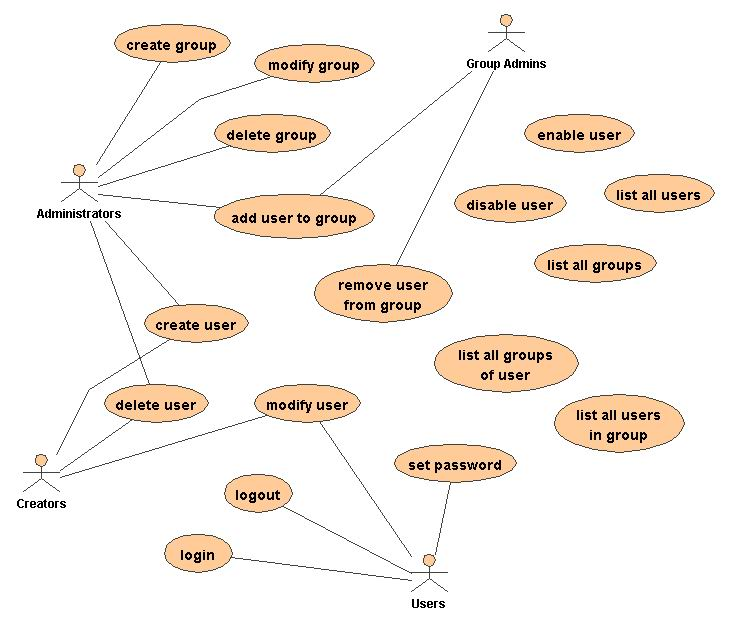
\includegraphics[scale=0.55]{ProgGuide_2User_UseCase.jpg}
    \caption{Gesch"aftsprozesse der Benutzerverwaltung in MyCoRe}
    \label{fig:UserUseCases}
  \end{center}
  \vspace{-1.4cm}
\end{figure} 

Offensichtlich d"urfen nicht alle Akteure des Systems die Berechtigung haben, alle 
Gesch"aftsprozesse durchf"uhren zu k"onnen. 
Daher muss ein System von Privilegien und Regeln implementiert werden: Benutzer/innen 
haben Privilegien (z.B. die Berechtigung, neue Benutzer/innen zu erstellen). 
Die Vergabe der Privilegien wird durch die Mitgliedschaft der Benutzer/innen in Gruppen 
geregelt. 
Dar"uber hinaus muss das System definierten Regeln gehorchen. 
So gen"ugt z.B. das Privileg "add user to group" allein nicht, 
um genau das Hinzuf"ugen eines Benutzers zu einer Gruppe definieren zu k"onnen. 
Die Regel ist in diesem Fall, dass ein Administrator jeden beliebigen Benutzer in 
jede beliebige Gruppe setzen kann, jeder andere Benutzer mit diesem Privileg aber maximal 
die Zugeh"origkeit zu Gruppen vergeben kann, in denen er or sie selbst Mitglied ist. 
Auf diese Weise wird verhindert, dass sich ein Benutzer oder eine Benutzerin selbst 
h"ohere Privilegien zuweisen kann. 
Die Privilegien und Regeln der MyCoRe-Benutzerverwaltung werden weiter unten ausf"uhrlich 
aufgef"uhrt.

\subsection{Benutzer, Gruppen, Privilegien und Regeln}
{\bf Benutzer}\\
Die Attribute von Benutzer/innen des Systems k"onnen in drei Bereiche klassifiziert 
werden, den account-Informationen wie ID, Passwort, Beschreibung usw., 
den Adress-Informationen wie Name, Anrede, Fakult"atszugeh"origkeit usw. sowie 
den Informationen "uber die Mitgliedschaft zu Gruppen. 
Die aktuell implementierten Benutzerattribute kann man an folgender beispielhafter 
XML-Darstellung erkennen:

{\bf to be continued ...}
